%----------------------------------------------------------------------------------------
%	INTRODUCTION
%----------------------------------------------------------------------------------------
\section{Introduction}
\label{ch:Introduction}

An essential step in the commercial asparagus cultivation is the sorting of the harvested asparagus into different quality classes. Depending on size, shape, and color, a label is assigned to the individual asparagus which determines the quality class of the asparagus~\citep{unspargelnorm}. Nowadays, this task is usually performed automatically, with modern asparagus sorting machines achieving a throughput of up to twelve asparagus spears per second~\citep{ting2015zeitalter}. However, the accuracy of such machines can be unsatisfying. Manual resorting is usually necessary and thereby causes substantial effort.

\bigskip
The aim of this study project was to investigate how techniques from computer vision, both classical and deep learning-based, can be applied to improve classification results for asparagus sorting machines. Asparagus is sorted by quality. The quality is defined based on several features that represent differences in color, shape, or texture. Hence, improving sorting algorithms for the classification of asparagus requires reliable means of measuring these features. As such, we were interested in the question of how the quality-defining features of asparagus can be estimated using state of the art computer vision and machine learning techniques.

The project was supported by a local asparagus farm and a company specializing in asparagus sorting machines. They provided training data and expertise on the classification of the asparagus. The idea to apply new machine learning approaches to a commercial problem of the agricultural industry seemed promising and challenging at the same time. As the data received from the farm was unlabeled, a larger focus on the preprocessing of the recorded image data became inevitable. Further, the variance in quality classes and the subjective view of human sorting behavior toughened the perspective on a practical application into the actual sorting machine. Nevertheless, the original goal of studying different techniques in computer vision and testing their usability in a fixed hardware setting for asparagus classification gave valuable insights into the practical application of previously theoretically assessed knowledge.

The hands-on experience on a long-term project gave us the chance to improve our project management skills, learn how to distribute work, and how to organize ourselves in a larger team. Over the course of one year, the team members worked on the implementation of different approaches to tackle the issue of image classification. After intense engagement with the subject, the methodologies and the project outcome were documented and critically reviewed. On the following pages, the different stages of the project together with the results of the applied computer vision approaches are described in detail. The report chapters are mostly in chronological order, each with the focus on a different stage of the study project throughout the year.

\bigskip
In chapter~\ref{ch:Introduction}~\nameref{ch:Introduction}, the idea of the project is presented together with an introduction to the current standards of image classification in machine learning as well as a general background on the quality classes, the sorting process, and classification of asparagus in the agricultural industry.

Chapter~\ref{ch:DataAcquisition}~\nameref{ch:DataAcquisition} comprises the process of data acquisition and organizational background to the project. This includes task management and teamwork, as well as a thorough evaluation of our planning abilities as a group. Further, the process of data collection and a first inspection of the sorting machine are elaborated, with an emphasis on the first issues of unlabeled data. There is not much literature on applying deep learning to agriculture. Still, our literature research gave an insight into practical possibilities and a rough guideline for our endeavor. The collected literature that was found to be close to our topic is reported at the end of this chapter.

In chapter~\ref{ch:Dataset}~\nameref{ch:Dataset}, the preprocessing phase is captured with the building of the data set at its end section. The first classical machine learning techniques for automatic feature extraction on image data are explored, followed by the process of manual feature extraction with the usage of a labeling application. The resulting outcome is reported, evaluated, and the labeled image data is transformed into a data set for the training of the chosen models.

Chapter~\ref{ch:Classification}~\nameref{ch:Classification} constitutes the different approaches that were chosen to tackle the issue of image classification. All approaches are critically reviewed and discussed in the subchapters. An emphasis was put on the application of deep learning techniques for the classification of the asparagus. As the collected data includes labeled and unlabeled samples, methods from the range of supervised learning, semi-supervised learning, and unsupervised learning were tested.

Chapter~\ref{ch:Summary}~\nameref{ch:Summary} contains the overall results of the classification approaches. The outcome of each approach is described and compared to the other methods as well as to the original classification accuracy of the sorting machine at the asparagus farm. Further, the overall results are discussed with an evaluation of their practical application in the food industry in chapter~\ref{ch:Discussion}~\nameref{ch:Discussion}. The overall outcome of the project is judged as a scientific study and as a team management experience.

In Chapter~\ref{ch:Conclusion}~\nameref{ch:Conclusion}, the findings are set into a broader perspective. The project and its results are summarized on a scientific basis as well as on an organizational level while the future prospects of the project are assessed.

\bigskip
Before analyzing the specific context of software development for the application in classification tasks further, a thorough insight into the idea of the study project is given in the following chapter. Additionally, background on the addressed topics of machine learning and the sorting of asparagus is provided.
In~\ref{sec:Project}~\nameref{sec:Project}, the objective of the study project is introduced. The next section~\ref{sec:BackgroundCV}~\nameref{sec:BackgroundCV}, gives an overview of the machine learning techniques that explore how image classification can be implemented and how these approaches can provide a solution to our issue. The first chapter concludes with~\ref{sec:BackgroundSortingAsparagus}~\nameref{sec:BackgroundSortingAsparagus}, where the process of asparagus classification in the commercial food industry is illustrated and the different quality classes of asparagus are defined.


\subsection{The project}
\label{sec:Project}

The objective of the study project was to find both, conventional and deep learning computer vision-based approaches that can be tested for their practical application in the commercial sorting of white asparagus. The different methods were implemented based on the image data that was received from the automatic sorting machine Autoselect ATS II employed by the asparagus farm ``Gut Holsterfeld’’~\footnote{see the website of Gut Holsterfeld at~\url{https://www.gut-holsterfeld.de/}}. It is explored whether approaches from the fields of machine learning and computer vision can be applied to improve the classification behavior of the asparagus sorting machine. Further it is investigated, if these approaches can be used in a more industrial than scientific setting for the specific task of asparagus classification. The initial intention to directly implement new software into the machine was postponed to allow for intensive research on the different approaches and on fine-tuning the received data to build a practical data set to train neural networks.

The idea for the project was formed by one of the students of the study group. She has a familial relationship to the asparagus farm Gut Holsterfeld and had received note of the unsatisfying classification performance of its sorting machine. The practical application to a real-world problem sparked the interest of the group and the general curiosity towards computer vision, in particular neural networks, further inspired to deal with the sorting issue in a deep learning context, as well as with classical methods.

All project members are students in the field of Cognitive Science at the University of Osnabr{\"u}ck. The study project is part of the Master Program in Cognitive Science at the University of Osnabr{\"u}ck. It is supervised by Dr.\ Ulf Krumnack and Axel Schaffland.

The study project intends to confirm the ability of its participants to independently formulate and solve an unknown problem from the scientific context of one subject area using the methods and terms they previously learned~\citep{moduledescription,studyregulations}. This includes the documentation and presentation of the results, the methodologies as well as the reflection on the work process. Within the scope of the project, for example, the development of software, analysis, and interpretation of statistical data material is practiced. A further aspect of the study project is to deepen the communicative and decision-making competence of its participants~\citep{moduledescription}. The idea is to train independent project work in groups of students under conditions that are common for research projects in science or industry.

As the project took part in the scope of an examination for the Cognitive Science Master Program at the University of Osnabr{\"u}ck, most of the work was developed at the university, that is, at the \acrfull{ikw}. 

Additional image data was received from the asparagus farm ``Querdel’s Hof’’~\footnote{see the website of Querdel’s Hof at~\url{https://www.querdel.de/}}. Further cooperation existed with the mechanical engineering company HMF Hermeler Maschinenbau GmbH~\footnote{see the website of HMF Hermeler at~\url{www.hmf-hermeler.de}} that developed the sorting machine Autoselect ATS~II and provided valuable expertise on the sorting issue.

All associated software is stored online, in our GitHub repository, and at the institute internal storing system.\footnote{The documentation to the project can be found at~\url{https://asparagus.readthedocs.io/en/latest}. The GitHub repository can be found at~\url{https://github.com/CogSciUOS/asparagus}. \\ Until 31/07/2020, the internal storing folder to the project at the University of Osnabr{\"u}ck could be accessed via~/net/projects/scratch/winter/valid\_until\_31\_July\_2020/asparagus. Since then, it can be accessed via~/net/projects/scratch/summer/valid\_until\_31\_January\_2021/jzerbe, until 31/01/2021.}


\subsection{Classification based on computer vision}
\label{sec:BackgroundCV}

In this chapter, the current standard of computer-based image classification is described. The main focus will be on \acrfullpl{ann} and classical computer vision techniques. A broad overview of relevant topics will be given and their importance for this project will be underlined.

Computer vision is a field of computer science that aims to automatically extract high-level understanding from image data and provide appropriate output. It is closely linked with machine learning, which describes the ability of a system to learn and improve from experience rather than being specifically programmed. Machine learning is frequently used to solve computer vision tasks.

\bigskip
Image classification is one of the main subfields of computer vision which gains a lot of attention in the scientific as well as the economic world. Besides the classical computer vision techniques that use algorithmic approaches to determine patterns, edges, and other points of interest that can help to classify images, artificial intelligence was introduced to the field in the 1960s \citep{szeliski2010computer}. Since then, more and more creative and complex artificial neural networks were introduced to solve numerous classification tasks, including the recognition of letters, faces, and street signs~\citep{mironczuk2018recent,balaban2015deep,stallkamp2011german}.

Some experts claim that artificial neural networks revolutionized the field of image classification, yielding better results than ever before~\citep{he2016deep,alexnet2012original}. More and more challenges, for example ImageNet \citep{russakovsky2015imagenet}, were introduced and computer scientists all over the world implemented creative solutions for the proposed problems. Additionally, influential companies like Google have a deep interest in finding solutions for image-based classification problems and push the research on these and related topics even further. In the era of optimization, computer-based classification became indispensable in many industries and also found its way into agriculture which is the field of interest in this study project.
In the following, a short introduction in both artificial neural networks and classical computer vision techniques is given which will span a bridge to our current classification problem.

\bigskip
Neural networks are used for image classification in many domains. In contrast to the algorithmic approaches, it is not determined by the programmer how and what exactly the neural network learns. A large amount of data is provided to the model, which then extracts relevant information to learn the classification task. However, what is relevant to the model is not necessarily relevant or interpretable to a human observer. This is one of the biggest disadvantages compared to classical computer vision approaches, which are understandable and, therefore, interpretable and adjustable. Another problem that comes along with this is that the bias for those approaches often does not lie in the code itself but in the data, which is by far more difficult to detect and surpass. For this reason, many people see artificial neural networks as a black box, which may yield great results but cannot be fully understood. Recent advances try to tackle that issue by systematically researching artificial intelligence with the aim of making it more explainable~\citep{tjoa2019survey,gilpin2018explaining}.

In image classification, usually \acrfullpl{cnn} are used \citep{geron2019hands,lecun1995convolutional}, which are loosely inspired by the visual cortex of the brain. The idea is that highly specialized components or filters learn a very specific task, which is similar to the receptive fields of neurons in the visual cortex~\citep{hubel1962receptive}. These components can then be combined to high-level features which, in turn, can be combined to objects that can be used for classification~\citep{geron2019hands,bishop2006pattern,lecun1995convolutional}. In \acrshortpl{cnn} this concept is implemented by several successive convolutional layers in which one or more filters are slid over the input, generating so-called feature maps. Each unit in one feature map looks for the same feature but in different locations of the input. In recent years, \acrshortpl{cnn} improved so much that they outperform humans in many classification tasks~\citep{russakovsky2015imagenet,KarpathyConvNet}.

\bigskip
Although machine learning exhibits very promising results and a lot of research and literature is available on the topic, many branches of industry still rely on traditional computer vision techniques in their implementation of image classification. This also applies to the asparagus sorting paradigm. To the best of our knowledge, no asparagus sorting machine is currently on the market that uses artificial intelligence for its classification algorithm.

Many classical computer vision algorithms aim to detect and describe points of interest in the input images that can be generalized to features. For these features, low-level attributes such as rapid changes in color or luminance can be used. In contrast to the features learned with the help of machine learning, these features are not specific to any training data set and therefore do not depend on it being well-constructed. Further, they are usually created in a way that is interpretable by humans which makes them very flexible and easily adaptable to specific use cases. This is why in some cases, traditional computer vision techniques can solve a problem much more efficiently than deep learning approaches.

One of the big advantages of deep learning algorithms is that they can extract underlying features from the data. In machine learning, it is essential to know about the components constructing a problem, whereas artificial neural networks have the ability to learn the features of the data, combine and correlate them and thus enable faster learning without an explicit command how to do so \citep{LeCun2015}.

\bigskip
In summary, both approaches have interesting implications for computer-based image classification tasks and provide promising techniques for our problem of asparagus classification. While we rely mostly on machine learning for the classification task itself, traditional computer vision algorithms are used to detect important features from the images.


\subsection{Background on sorting asparagus}
\label{sec:BackgroundSortingAsparagus}

In this section, a background on sorting asparagus is given with a focus on the quality classes assessed by the asparagus farm Gut Holsterfeld. The owner of the asparagus farm, Mr. Silvan Schulze-Weddige, and the CEO of the engineering company HMF Hermeler Maschinenbau, Mr. Thomas Hermeler, were consulted on this issue.

\bigskip
While asparagus accounts for a fifth of the area used for vegetable cultivation in Germany, the harvesting season of white asparagus only spans over a period of two months, beginning in April and ending on the 24th of June ~\citep{spargelstatistik,nrw2018spargel}. During this period, the asparagus is harvested, classified, and sold in accord with a price range that is defined by the quality class of the asparagus.

\begin{table}[!ht]
	\centering
	\resizebox{\textwidth}{!}{%
	\begin{tabular}{l p{14cm}}
		\textbf{Label} & \textbf{Description} \\
		\noalign{\smallskip}
		\hline
		\\
		I A Anna & Quality class Extra is represented by I~A~Anna, I~A~Bona, and I~A~Clara. I~A is defined as asparagus that is perfectly straight and white. There are no large pressure marks, no rust, no violet color, and no curvature. The identification label Anna marks that the width (diameter) of the spear is in a range of 20 - 26 mm. \\
		\smallskip
		I A Bona & Quality class Extra asparagus with a width of width 18 - 20 mm. \\
		\smallskip
		I A Clara & Quality class Extra asparagus with a width of 16 - 18 mm. \\
		\smallskip
		I A Krumme & The asparagus fulfills all criteria for quality class Extra while it shows a slight curvature.\\
		\smallskip
		I A Violett & The asparagus is of a violet complexion, while it complies with all             guidelines for quality class Extra. The color change is due to the spear having contact with sunlight before being harvested. \\
		\smallskip
		II A & The asparagus is both curved and violet. \\
		\smallskip
		II B & The asparagus is curved, rusty, and/or in any other way damaged or 					classified as a defective product. \\
		\smallskip
		Rost & The asparagus shows traces of rust or has rusty parts that occur when the roots of the plant were injured in a preceding year. This should not be confused with a fungal disease that can also be referred to as rust. \\
		\smallskip
		Dicke & The asparagus exceeds 26 mm in width. \\
		\smallskip
		Hohle & The asparagus is hollow from the inside. \\
		\smallskip
		Blume & The head region of the asparagus is about to bloom or it shows clear 					outlines of a flower. \\
		\smallskip
		Suppe & The asparagus has a width of less than 16 mm. \\
		\smallskip
		Bruch & Any asparagus that is below a length of 210 mm. However, another                         distinction in this class label is made between asparagus that has an intact head and         a length of at least 100 mm (Kerze), asparagus without head (Bruch), and an                 asparagus head alone (K{\"o}pfchen).  \\
		\smallskip
		Keule & The upper end of the asparagus is thicker than the lower end. The shape                 is similar to a club, hence the name of the class. This class label was of no concern         to the project because no image data of this class label could be recorded. \\
		\\
		\hline
	\end{tabular}%
	}
	\caption[List of Asparagus Quality Classes]{\textbf{List of Asparagus Quality Classes}~~~In this table, 14 quality classes for asparagus categorization are listed and described, according to the asparagus farm Gut Holsterfeld. Except for the class label Keule, all 13 quality classes were used as the goal label for the asparagus classification.}
	\label{tab:AsparagusLabels}
\end{table}

In the European Union, there is a uniform system for the sorting of asparagus into quality classes~\citep{euspargelnorm,unspargelnorm}.\footnote{see \url{https://mlr.baden-wuerttemberg.de/de/unser-service/presse-und-oeffentlichkeitsarbeit/pressemitteilung/pid/nationale-handelsklassen-fuer-frisches-obst-und-gemuese-abgeschafft-1/}}\footnote{see \url{https://www.bzfe.de/inhalt/spargel-kennzeichnung-5876.html}} However, supply and demand usually determine the number and accuracy of these classes. One of the first defining features is the color of the asparagus which comprises four categories: white, violet, violet-green, and green~\citep{euspargelnorm}. For this project, only the first two colors are of relevance. A further distinction is made between the quality classes Extra, class I, and class II. The class Extra defines the product as perfect quality, class I defines it as good quality, and class II includes products that do not qualify for the other classes but satisfy the minimum requirements for commercial distribution~\citep{euspargelnorm}. The last distinction is made for the characteristics of length and width. White and violet asparagus may not exceed 220 mm in length. The minimal length of the asparagus varies but should be above 170 mm for long asparagus. Additionally, there is some level of tolerance accepted for the quality classes. According to the quality class, 5\% - 15\% of wrongly sorted asparagus is tolerated in a package or bundle~\citep{euspargelnorm}.

\begin{figure}[!b]
	\centering
	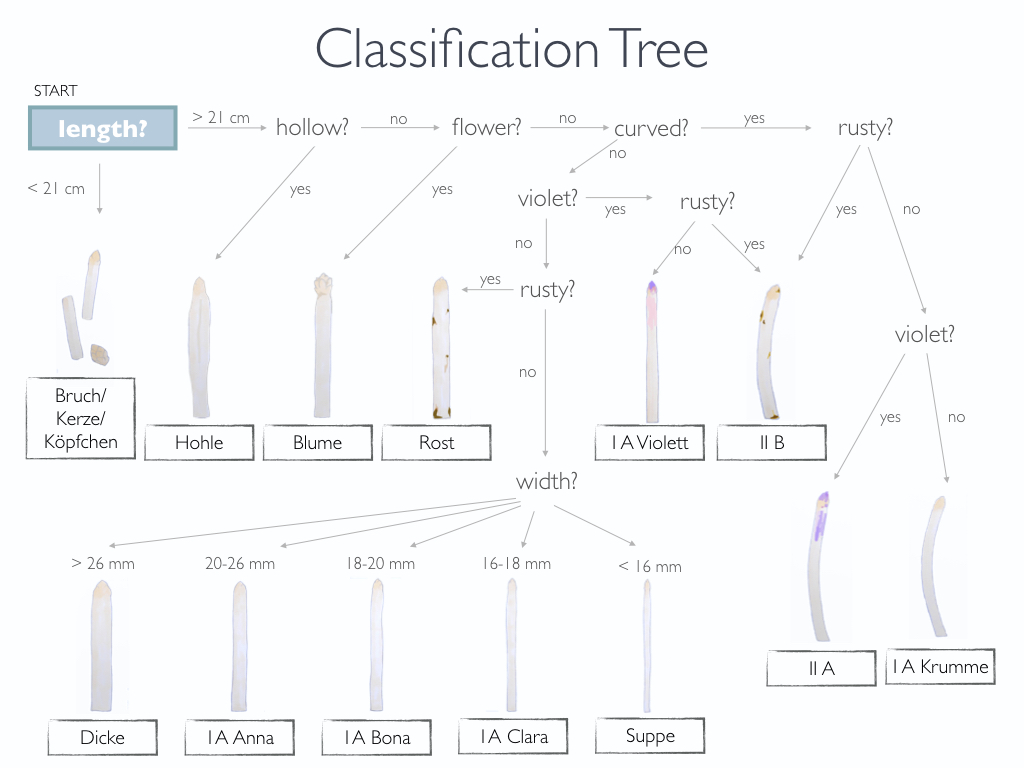
\includegraphics[scale=0.39]{Figures/chapter01/treewithtitle.png}
	\decoRule
	\caption[Asparagus Classification Tree]{\textbf{Asparagus Classification Tree}~~~The classification tree shows how each asparagus is attributed with a label of its quality class. It was drawn by the project group and follows the sorting rules of the asparagus farm Gut Holsterfeld. Starting from the upper left corner of the image, mostly binary decisions are made until a label is reached. Any further damaged or defective asparagus automatically belongs in category II~B.}
	\label{fig:LabelTree}
\end{figure}

\bigskip
Depending on how carefully the individual farmer further categorizes the asparagus, additional classes can be established. Regional differences to those classes make the challenge for the manufacturers of sorting machines even more complicated. The class labels as stated in this report depend solely on the sorting conduct of the asparagus farm Gut Holsterfeld and do not necessarily apply to any other classification system of the asparagus industry.

In~\autoref{tab:AsparagusLabels}, 14 quality classes are shortly described, of which 13 classes are relevant to this project. The classification tree in~\autoref{fig:LabelTree} illustrates the decision process that underlies the categorization of the relevant classes.

\bigskip
One of the challenges of asparagus classification with a machine lies in the human sorting error. The machine can assess exact calculations about, for example, the length or the width of a spear, while the human observer might not be able to detect minor differences in these features. Thus, a threshold has to be defined if a spear is sorted into a certain class. However, the data on which the machine calculates its features to characterize an asparagus spear was previously labeled by a human. The sorter might miss subtle differences in color. For example, the machine might sort a spear as the class label Violett while the spear would be judged as the class label I A Anna by the human sorter. Since human sorting behavior is subjective, the same asparagus can be categorized differently by two independent sorters. Furthermore, asparagus sorted twice by the same person at different time points might be assigned with two different class labels.

A second problem for the sorting machine poses the interpretation of colors. The color can be perfectly recognized by its program, however, the structure of the color is also important for correct classification. The machine might not be able to distinguish whether the asparagus was, e.g.\ of brownish color because it is very rusty or simply very dirty in certain cases.

A third factor for classification difficulties is caused by the restricted view of the product. Asparagus can look perfectly shaped from one angle but might be damaged on the side that is not exposed to the camera of the sorting machine.

Another complication poses the question of demand and supply. During some seasons there is more asparagus of a certain class label and less of another one available. The farmer usually distributes the number of spears belonging to a quality class according to the seasonal conditions. For example, during a season with less high-quality asparagus of the classes I~A, the sorting threshold will shift. Spears that are usually sorted into, e.g.\ a lower class will now belong to a higher quality class. The challenge for a sorting machine will not only be to sort for the class criteria but also to provide a flexible and individual solution in accordance with the preferences of the farmer.

These challenges are not impossible to overcome but they make it more difficult to find a solution to the sorting task and compromises in the implementation (f.e.\ the precision of classification) might be necessary. 
